\section{Speech Emotion Recognition}
Another key element of Pookie’s AI is the Speech Emotion Recognition (SER) system, which is used for recognizing the user’s emotions based on vocal patterns. By analyzing factors such as pitch, tone, and intensity, the system detects emotions: neutral, anger, happiness, sadness, and frustration. This section outlines the current progress, challenges, and future approaches for designing the speech emotion recognition model, including relevant datasets and methodologies.
\subsection{Speech Emotion Recognition Model}
We are utilizing a dataset created by Chulalongkorn University in collaboration with VISTEC, DEPA, and AIS, containing 41 hours and 36 minutes of audio recordings labeled with five emotions: neutral, anger, happiness, sadness, and frustration. VISTEC has also developed a speech emotion recognition model based on this dataset. We are in the process of adjusting the model's parameters to better fit our system.

\subsubsection*{Parameters:}

\begin{itemize}
    \item \textbf{Number of Mel-filterbanks:} Mel-filterbanks are used to transform the frequency spectrum into a scale that better aligns with how humans perceive sound. By adjusting the number of filterbanks, we can control the resolution of this transformation, which affects the granularity of frequency representation in the model. More filter banks provide finer detail, while fewer filterbanks reduce the model’s sensitivity to frequency variations.
    \item \textbf{Sampling Rate:} The sampling rate refers to how many samples per second the audio is recorded or processed. A higher sampling rate captures more detail from the audio signal, but it also increases the computational load. Adjusting this parameter ensures that the audio quality is sufficient for emotion recognition without overwhelming system resources.
    \item \textbf{Frame Length of STFT:} The STFT converts audio signals into a time-frequency representation. The frame length defines how long each segment of audio is for this transformation. A longer frame provides more frequency resolution but less time precision, while a shorter frame offers better time resolution but less frequency detail. Balancing these is key for accurate emotion recognition.
    \item \textbf{Epochs:} This parameter refers to the number of times the entire training dataset passes through the model during training. Adjusting the number of epochs affects how well the model learns from the data. Too few epochs may lead to underfitting, where the model doesn’t learn enough, while too many can cause overfitting, where the model memorizes the training data but performs poorly on new data.

\end{itemize}

The results are as shown in Figure 3, Figure 4, and Figure 5.

\begin{figure}[ht]
    \centering
    \captionsetup{justification=centering}
    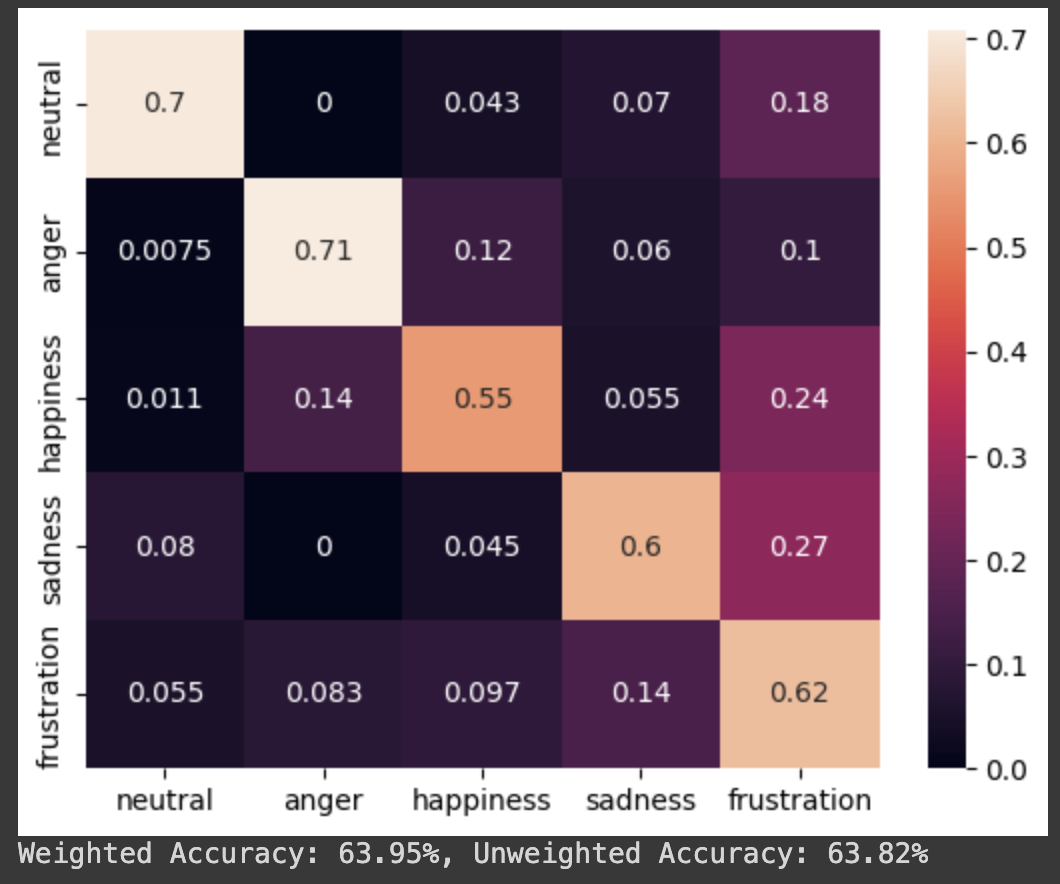
\includegraphics[width=0.5\textwidth]{default.png}
    \caption{Default parameters with 80 mel-filterbanks, sampling rate at 16,000 Hertz, and frame length of STFT at 50 milliseconds at 80 epochs}
    \label{fig:default}
\end{figure}

\begin{figure}[ht]
    \centering
    \captionsetup{justification=centering}
    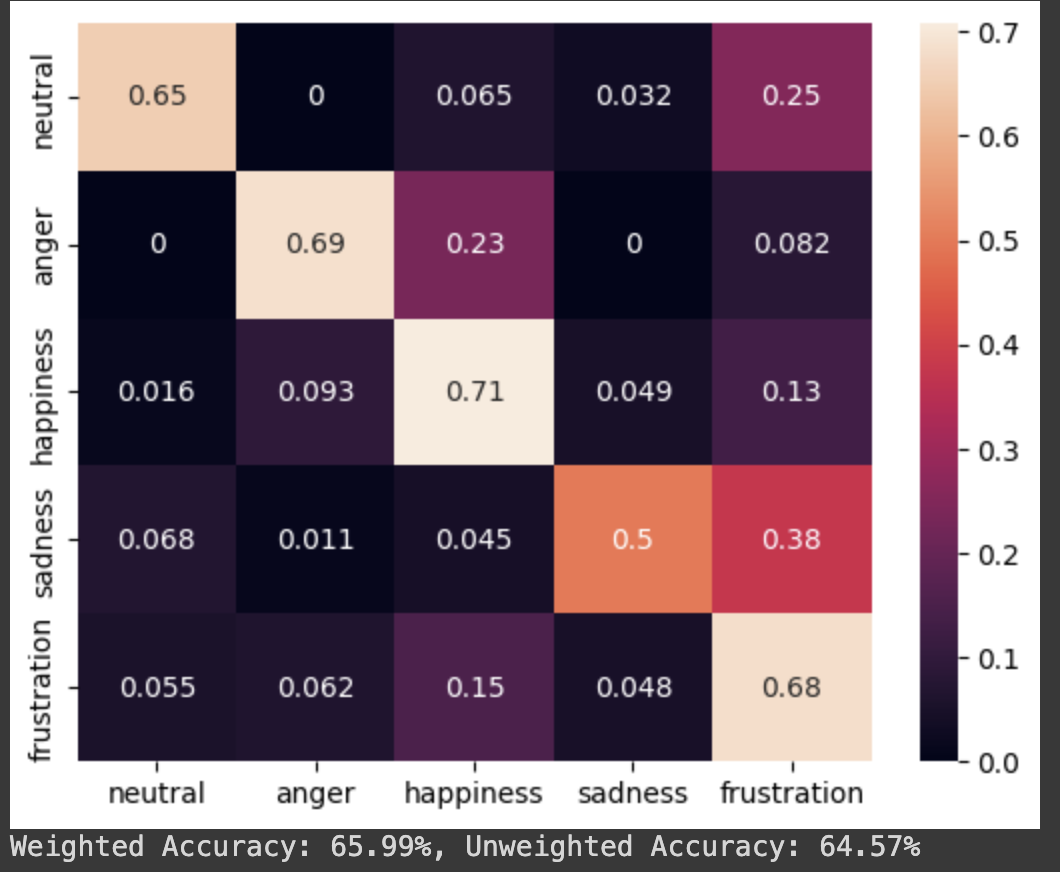
\includegraphics[width=0.5\textwidth]{128m-22050.png}
    \caption{Tuned model with 128 mel-filterbanks, sampling rate at 22,050 Hertz, and frame length of STFT at 50 milliseconds at 60 epochs}
    \label{fig:128m-22050}
\end{figure}

\begin{figure}[ht]
    \centering
    \captionsetup{justification=centering}
    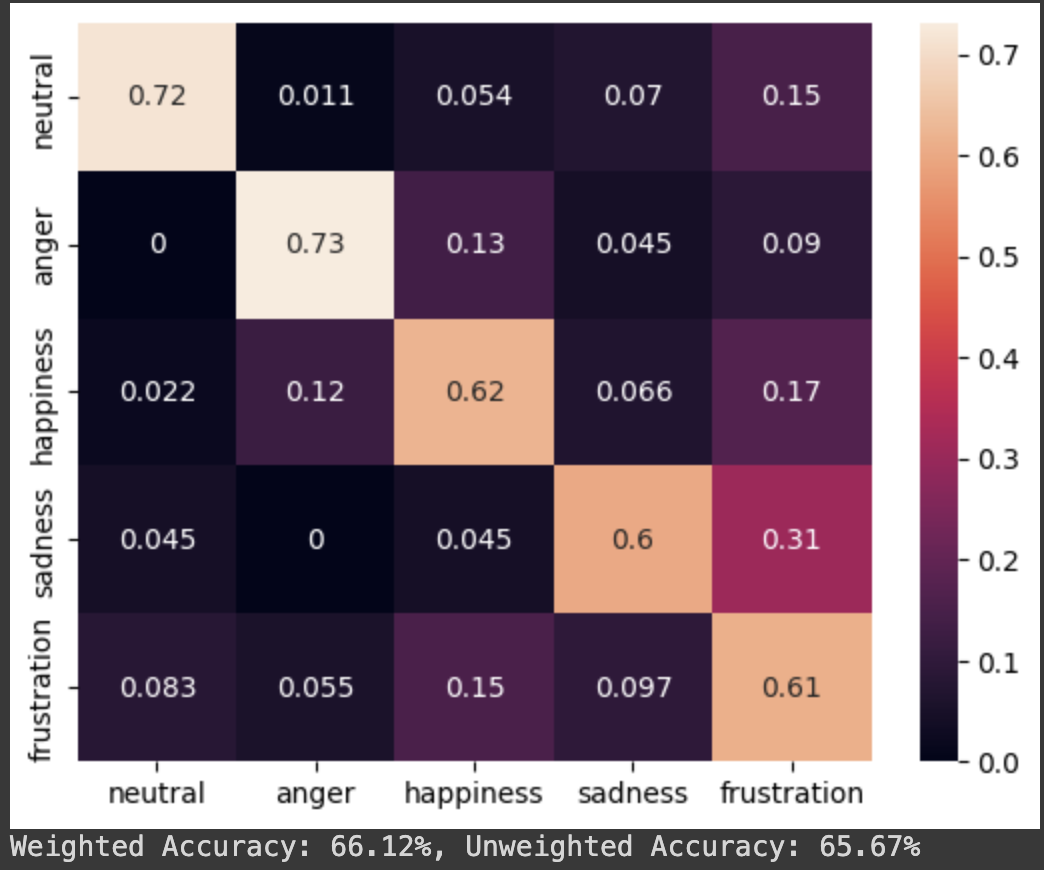
\includegraphics[width=0.5\textwidth]{128m-25ms.png}
    \caption{Tuned model with 128 mel-filterbanks, sampling rate at 16,000 Hertz, and frame length of STFT at 25 milliseconds at 60 epochs}
    \label{fig:128m-25ms}
\end{figure}

\subsection{Design Challenges}
Similarly to the FER, the input-output interaction for SER also poses a significant challenge:
\begin{itemize}
    \item \textbf{Defining input/output structure:} This design challenge which was addressed for FER is also present in SER as these two systems are intertwined and SER’s initialization might depend on other factors such as duration of facial detection. As of the report this is still under discussion as mentioned in the FER section.
\end{itemize}
    
    Overall, the current design issues of the SER stems from undecided input and output structure and interactions, both of which will be addressed by the next progress report in October.

\subsection{Technical Challenges}
Several technical challenges have emerged, primarily related to compatibility:
\begin{itemize}
    \item \textbf{Compatibility issues:} The original SER model was created three years ago, and since then, Google Colab has updated its Python version from 3.7 to 3.10, alongside a CUDA update to version 12.1. Python 3.7 reached its end of life (EOL) as of June 27, 2023, which has caused compatibility issues with the model's required libraries. The mismatch between Google Colab’s Python environment and the model’s requirements has led to several errors. To address this, we created a forked version of the original VISTEC-SER model and modified it according to the updated dependencies which include a plethora of changes to the source code.
\end{itemize}